\ifx\wholebook\relax\else
\documentclass[twoside]{book}
\usepackage[active]{srcltx}
\usepackage[LY1]{fontenc}
\usepackage{epsfig}
\def\etc{{\it etc}}
\def\eg{{\it e.g.}}
\def\ie{{\it i.e.}}
\def\cf{{\it c.f.}\ }
\def\erf{\mathop{\rm erf}}
\def\sign{\mathop{\rm sign}}
\def\prob{\mathop{\rm Prob}}
\def\var{\mathop{\rm var}}
\def\mod{\mathop{\rm mod}}
\def\cor{\mathop{\rm cor}}
\def\cov{\mathop{\rm cov}}
\def\cl{\mathop{\rm CL}}
\def\kg{\mathop{\rm Kg}}
\def\patstyle#1{{\sc #1}}
\def\th{^{\mathop{\rm th}}}
\def\st#1{^{\mathop{\rm #1}}}
\def\note#1{\begin{quote}{\bf Note:} #1\end{quote}}
\def\braket#1{\left\langle #1\right\rangle}
\def\order#1{\let\o=#1{\cal O}\ifx\o 1$\left(n\right)$\else$\left(n^{#1}\right)$\fi}
\newtheorem{privListing}{Listing}[chapter]
\newenvironment{listing}{\vskip 3ex\hrule\vskip 1ex\begin{privListing}}{\end{privListing}\hrule\vskip 1ex}
\newtheorem{privExample}{Code example}[chapter]
\newenvironment{codeExample}{\begin{privExample}\begin{quote}\tt}{\end{quote}\end{privExample}}
\def\relboxl#1#2{\hbox to #1\hsize{#2\hfil}}
\def\relboxc#1#2{\hbox to #1\hsize{\hfil #2\hfil}}
\def\relboxr#1#2{\hbox to #1\hsize{\hfil #2}}
\def\transpose#1{{\bf #1}^{\mathop{\rm T}}}
\def\inverse#1{{\bf #1}^{-1}}
%\def\tm{$^{\mathop{\rm TM}}$}
\def\tm{ }
\newenvironment{mainEquation}{\marginpar[\vspace{3 ex} Main
equation$\Rightarrow$]{\vspace{3 ex}$\Leftarrow$Main
equation}\begin{equation}}{\end{equation}}
\def\rubrique#1{\paragraph{#1}\hfil\par\noindent}

\begin{document}
\fi

\chapter{Finding the zero of a function}
\label{ch:zeroes} \vspace{1 ex}
\begin{flushright} {\sl Le z\'ero, collier du n\'eant.}\footnote{The zero, a necklace for emptiness.}\\ Jean Cocteau
\end{flushright}
\vspace{1 ex}
The zeroes of a function are the values of the
function's variable for which the value of the function is zero.
Mathematically, given the function $f\left(x\right)$, $z$ is a
zero of when $f\left(z\right)=0$. This kind of problem is can be
extended to the general problem of computing the value of the
inverse function, that is finding a value $x$ such that
$f\left(x\right)=c$ where $c$ is a given number. The inverse
function is noted as $f^{-1}\left(x\right)$. Thus, one wants to
find the value of $f^{-1}\left(c\right)$ for any $c$. The problem
can be transformed into the problem of finding the zero of the
function $\tilde{f}\left(x\right)=f\left(x\right)-c$.

The problem of finding the values at which a function takes a
maximum or minimum value is called searching for the extremes of a
function. This problem can be transformed into a zero-finding
problem if the derivative of the function can be easily computed.
The extremes are the zeroes of the function's derivative.

\noindent Figure \ref{cl:zeroFinding} shows the class diagram of
the classes discussed in this chapter.
\begin{figure}
\centering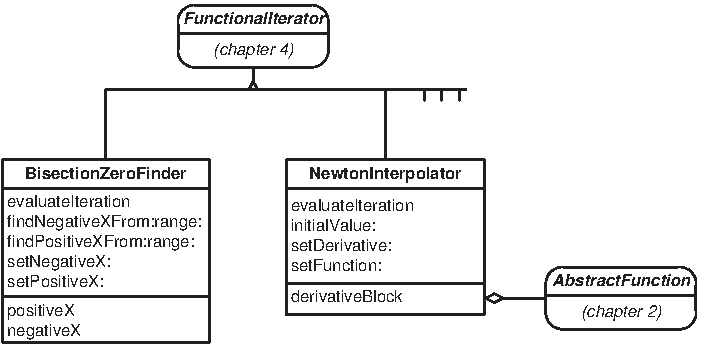
\includegraphics[width=10cm]{Figures/ZeroClassDiagram}
\caption{Class diagram for zero finding
classes}\label{cl:zeroFinding}
\end{figure}


\section{Introduction}
Let us begin with a concrete example.

Often an experimental result is obtained by measuring the same
quantity several times. In scientific publications, such a result
is published with two numbers: the average and the standard
deviation of the measurements. This is true for medical
publication as well. As we have already discussed in section
\ref{sec:errorFunctionDef}, obstetricians prefer to think in terms
of risk and prefer to use centiles instead of average and standard
deviation. Assuming that the measurements were distributed
according to a normal distribution (\cf section
\ref{sec:normdist}), the 90th centile is the solution to the
following equation:
\begin{equation}
\label{eq:centile90}
  \erf\left(x\right)=0.9
\end{equation}
That is, we need to find the zero of the function
$f\left(x\right)=\erf\left(x\right)-0.9$. The answer is $x=1.28$
with a precision of two decimals. Thus, if $\mu$ and $\sigma$ are
respectively the average and standard deviation of a published
measurement, the 90th centile is given by $\mu+1.28\cdot\sigma$.
Using equation \ref{eq:erfneg} the 10th centile is given by
$\mu-1.28\cdot\sigma$.

\section{Finding the zeroes of a function --- Bisection method}
\label{sec:bisection}\marginpar{Figure \ref{cl:zeroFinding} with
the box {\bf BisectionZeroFinder} grayed.} Let assume that one
knows two values of $x$ for which the function takes values of
opposite sign. Let us call $x_{\mathop{\rm pos}}$ the value such
that $f\left(x_{\mathop{\rm pos}}\right)>0$ and $x_{\mathop{\rm
neg}}$ the value such that $f\left(x_{\mathop{\rm neg}}\right)<0$.
If the function is continuous between $x_{\mathop{\rm pos}}$ and
$x_{\mathop{\rm neg}}$, there exists at least one zero of the
function in the interval $\left[ x_{\mathop{\rm
pos}},x_{\mathop{\rm neg}}\right]$. This is illustrated in figure
\ref{fig:bisection}. If the function $f$ is not continuous over
the interval where the sign of the function changes, then the
presence of a zero cannot be guaranteed\footnote{The inverse
function is such an example. It changes sign over 0 but has no
zeroes for any finite $x$}. The continuity requirement is
essential for the application of the bisection algorithm.

The values $x_{\mathop{\rm pos}}$ and $x_{\mathop{\rm neg}}$ are
the initial values of the bisection algorithm. The algorithm goes
as follows:
\begin{enumerate}
  \item Compute $x={x_{\mathop{\rm pos}}-x_{\mathop{\rm neg}}\over
  2}$.
  \item If $f\left(x\right)>0$, set $x_{\mathop{\rm pos}}=x$ and
  goto step 4.
  \item Otherwise set $x_{\mathop{\rm neg}}=x$.
  \item If $\left|
x_{\mathop{\rm pos}},x_{\mathop{\rm neg}}\right|>\epsilon$ go back
to step 1. $\epsilon$ is the desired precision of the solution.
\end{enumerate}
The first couple of steps of the bisection algorithm are
represented geometrically on figure \ref{fig:bisection}. Given the
two initial values, $x_{\mathop{\rm pos}}$ and $x_{\mathop{\rm
neg}}$, the first iteration of the algorithm replaces
$x_{\mathop{\rm pos}}$ with $x_1$. The next step replaces
$x_{\mathop{\rm neg}}$ with $x_2$.
\begin{figure}
\centering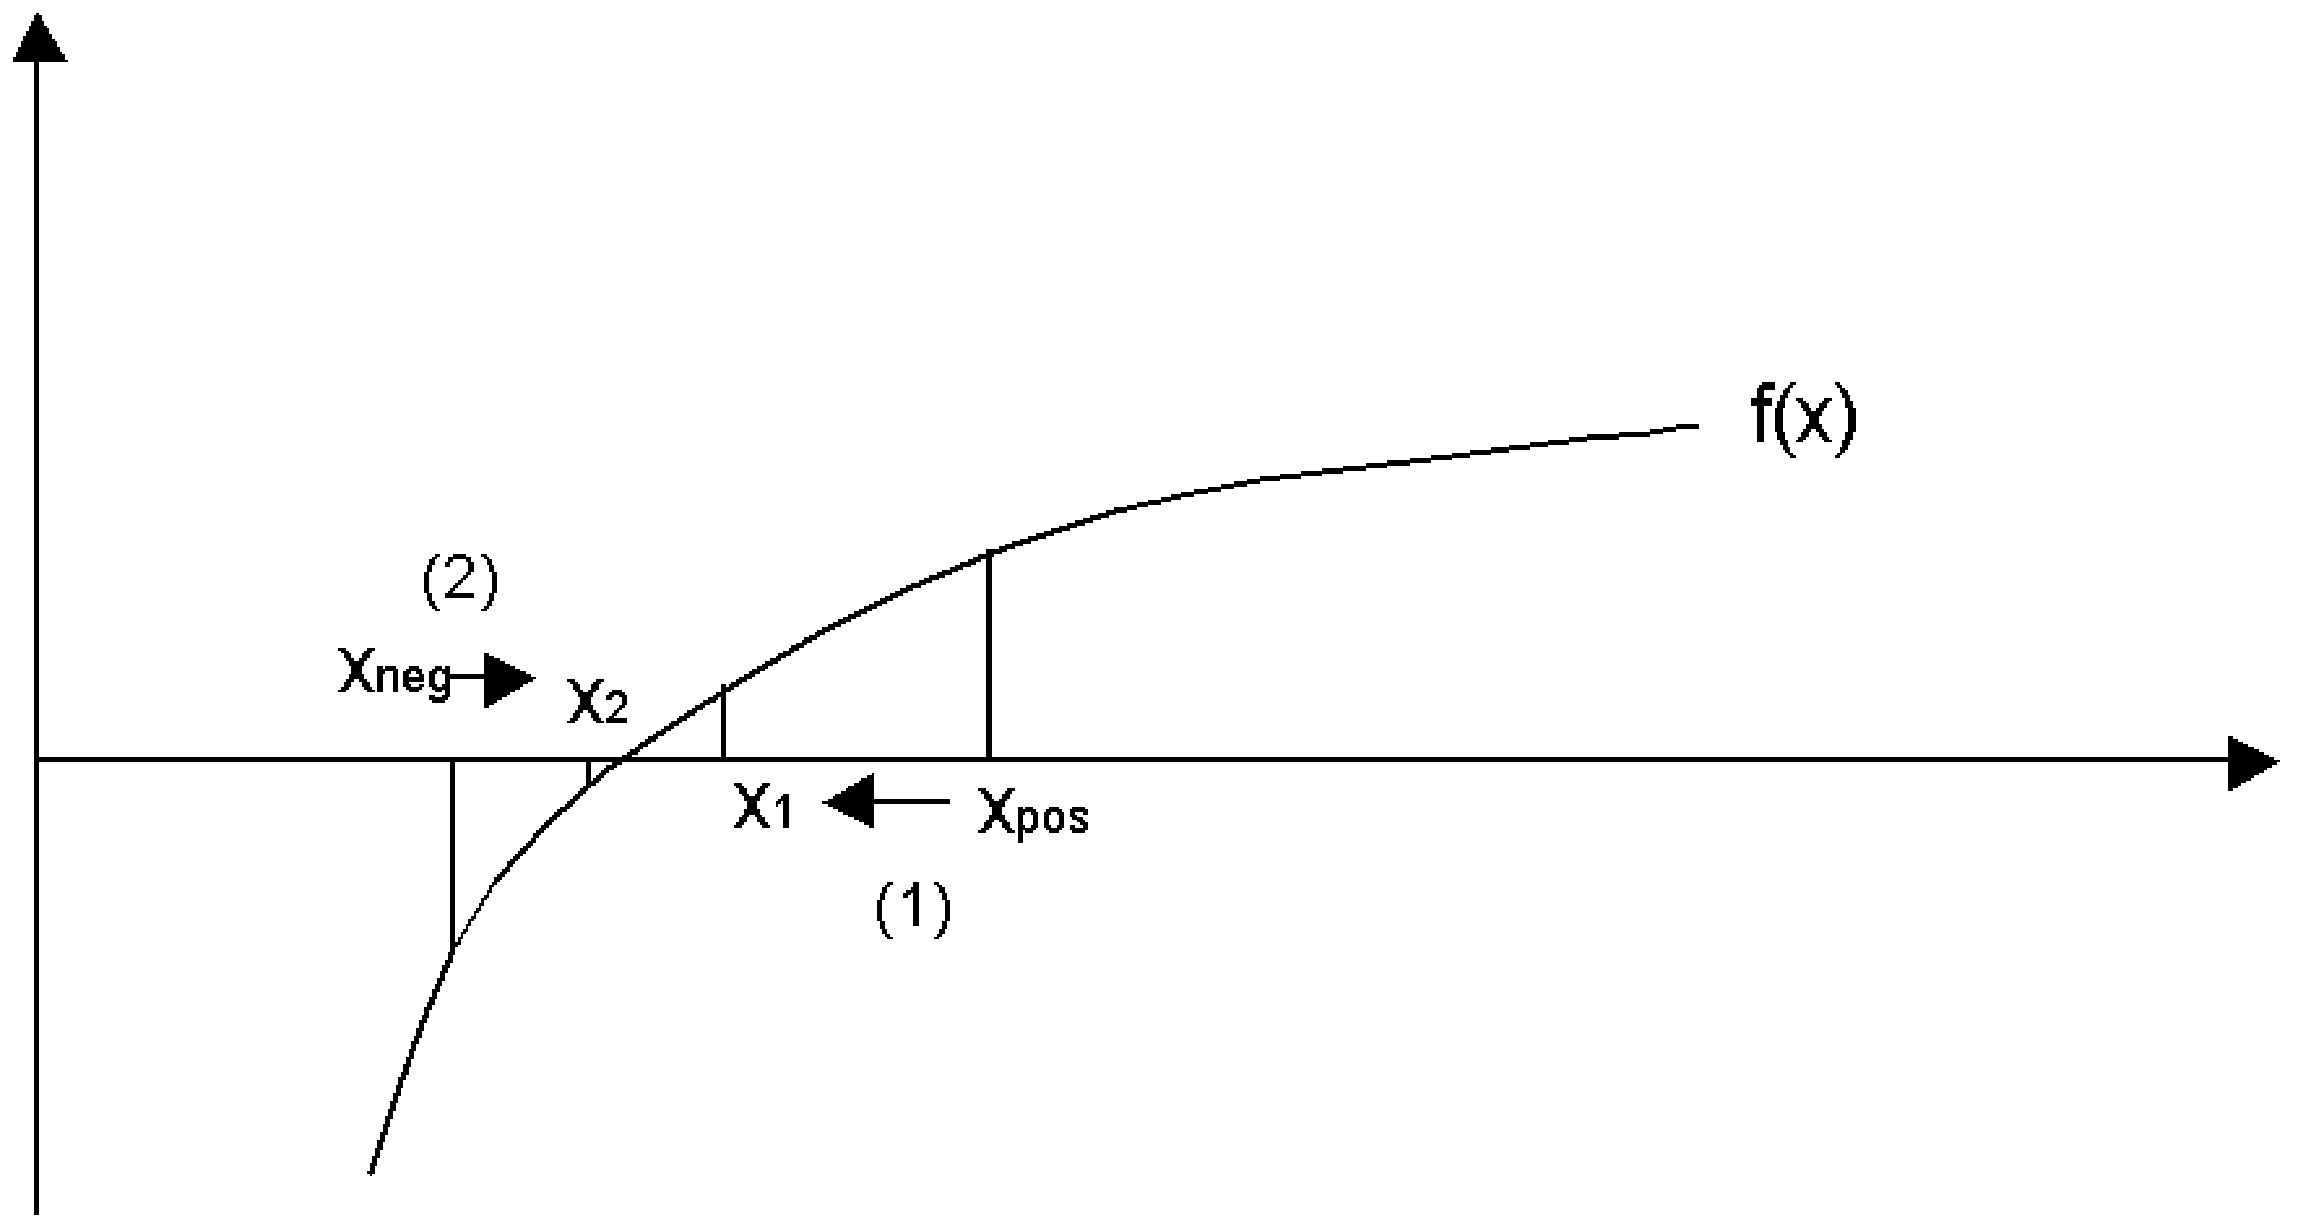
\includegraphics[width=12cm]{Figures/BissectionGraph}
\caption{The bisection algorithm}\label{fig:bisection}
\end{figure}

For a given pair of initial values, $x_{\mathop{\rm pos}}$ and
$x_{\mathop{\rm neg}}$, the number of iterations required to
attain a precision $\epsilon$ is given by:
\begin{equation}
\label{eq:bissectime}
  n=\left\lceil\log_2{\displaystyle\left|
x_{\mathop{\rm pos}},x_{\mathop{\rm neg}}\right| \over
\displaystyle\epsilon}\right\rceil.
\end{equation}
For example if the distance between the two initial values is 1
the number of iterations required to attain a precision of
$10^{-8}$ is 30. It shows that the bisection algorithm is rather
slow.

Knowledge of the initial values, $x_{\mathop{\rm pos}}$ and
$x_{\mathop{\rm neg}}$, is essential for starting the algorithm.
Methods to define them must be supplied. Two convenience methods
are supplied to sample the function randomly over a given range to
find each initial value. The random number generator is discussed
in section \ref{sec:random}.

The bisection algorithm is a concrete implementation of an
iterative process. In this case, the method {\tt
evaluateIteration} of figure \ref{fig:itermeth} implements steps
2, 3 and 4. The precision at each iteration is $\left|
x_{\mathop{\rm pos}}-x_{\mathop{\rm neg}}\right|$ since the zero
of the function is always inside the interval defined by
$x_{\mathop{\rm pos}}$ and $x_{\mathop{\rm neg}}$.

\subsection{Bisection algorithm --- General  implementation}

The class of the object implementing the bisection algorithm is a
subclass of the abstract class {\tt FunctionalIterator}. The class
{\tt BisectionZeroFinder} needs the following additional instance
variables.
\begin{description}
  \item[\tt positiveX]$x_{\mathop{\rm pos}}$ and
  \item [\tt negativeX]$x_{\mathop{\rm neg}}$
\end{description}
The bisection algorithm proper is implemented only within the
method {\tt evaluateIteration}. Other necessary methods have
already been implemented in the iterative process class.

\subsection{Bisection algorithm --- Smalltalk  implementation}
Finding the zero of a function is performed by creating an
instance of the class {\tt DhbBisectionZeroFinder} and giving the
function as the argument of the creation method as explained in
section \ref{sec:siterrel}. For example the following code finds
the solution of equation \ref{eq:centile90}.
\begin{codeExample}
\begin{verbatim}

 | zeroFinder result |
 zeroFinder:= DhbBisectionZeroFinder function: [ :x | x errorFunction - 0.9].
 zeroFinder setPositiveX: 10; setNegativeX: 0.
 result := zeroFinder evaluate. zeroFinder
 hasConverged
\end{verbatim}
    {\tt\hspace{4 em}ifFalse:[ {\sl <special case processing>}].}
\end{codeExample}
The second line creates the object responsible to find the zero.
The third line defines the initial values, $x_{\mathop{\rm pos}}$
and $x_{\mathop{\rm neg}}$. The fourth line performs the algorithm
and stores the result if the algorithm has converged. The last two
lines check for convergence and take corrective action if the
algorithm did not converge.

Listing \ref{ls:bisection} shows the implementation of the
bisection zero finding algorithm in Smalltalk.

The class {\tt DhbBisectionZeroFinder} is a subclass of the class
{\tt DhbFunctionalIterator}. As one can see only a few methods
need to be implemented. Most of them pertain to the definition of
the initial interval. In particular, convenience methods are
supplied to find a positive and negative function value over a
given interval.

The methods defining the initial values, $x_{\mathop{\rm pos}}$
and $x_{\mathop{\rm neg}}$, are {\tt setPositiveX:} and {\tt
setNegativeX:} respectively. An error is generated in each method
if the function's value does not have the proper sign. The
convenience methods to find random starting values are
respectively {\tt findPositiveXFrom:range:} and {\tt
findNegativeXFrom:range:}. The method {\tt computeInitialValues}
does not compute the initial values. Instead it makes sure that
$x_{\mathop{\rm pos}}$ and $x_{\mathop{\rm neg}}$ have been
properly defined.

\begin{listing} Smalltalk implementation of the bisection algorithm \label{ls:bisection}
$$\halign{ #\hfil&\quad#\hfil\cr {\sl Class}& {\Large\bf DhbBisectionZeroFinder}\cr
{\sl Subclass of }&{\tt DhbFunctionalIterator}\cr\noalign{\vskip 1ex}

{\sl Instance variable names:}&\parbox[t]{4 in}{\tt  positiveX negativeX }\cr\noalign{\vskip 1ex}}$$


Instance methods
{\parskip 1ex\par\noindent}
{\bf computeInitialValues}
\begin{verbatim}
    positiveX isNil
        ifTrue: [ self error: 'No positive value supplied'].
    negativeX isNil
        ifTrue: [ self error: 'No negative value supplied'].

\end{verbatim}
{\bf evaluateIteration}
\begin{verbatim}
    result := ( positiveX + negativeX) * 0.5.
    ( functionBlock value: result) > 0
        ifTrue: [ positiveX := result]
        ifFalse:[ negativeX := result].
    ^self relativePrecision: ( positiveX - negativeX) abs

\end{verbatim}
{\bf findNegativeXFrom:} {\tt aNumber1} {\bf range:} {\tt aNumber2}
\begin{verbatim}
    | n |
    n := 0.
    [ negativeX := Number random * aNumber2 + aNumber1.
      ( functionBlock value: negativeX) < 0
        ] whileFalse: [ n := n + 0.1.
                        n > maximumIterations
                            ifTrue: [ self error: 'Unable to find a 
                                            negative function value'].
                      ].

\end{verbatim}
{\bf findPositiveXFrom:} {\tt aNumber1} {\bf range:} {\tt aNumber2}
\begin{verbatim}
    | n |
    n := 0.
    [ positiveX := Number random * aNumber2 + aNumber1.
      ( functionBlock value: positiveX) > 0
        ] whileFalse: [ n := n + 1.
                        n > maximumIterations
                            ifTrue: [ self error: 'Unable to find a 
                                            positive function value'].
                      ].

\end{verbatim}
{\bf setNegativeX:} {\tt aNumber}
\begin{verbatim}
    ( functionBlock value: aNumber) < 0
        ifFalse:[ self error: 'Function is not negative at x = ', 
                                                 aNumber printString].
    negativeX := aNumber.

\end{verbatim}
{\bf setPositiveX:} {\tt aNumber}
\begin{verbatim}
    ( functionBlock value: aNumber) > 0
        ifFalse:[ self error: 'Function is not positive at x = ', 
                                                 aNumber printString].
    positiveX := aNumber.

\end{verbatim}


\end{listing}


\section{Finding the zero of a function --- Newton's method}
\label{sec:newton}\marginpar{Figure \ref{cl:zeroFinding} with the
box {\bf NewtonZeroFinder} grayed.} Isaac Newton has designed an
algorithm working by successive approximations\cite{Bass}. Given a
value $x_0$ chosen in the vicinity of the desired zero, the
following series:
\begin{mainEquation}
\label{eq:newtonZero}
  x_{n+1}=x_n-{f\left(x_n\right)\over f^{\prime}\left(x_n\right)},
\end{mainEquation}
where $f^{\prime}\left(x\right)$ is the first derivative of
$f\left(x\right)$, converges toward a zero of the function  . This
algorithm is sometimes called Newton-Ralphson\cite{Press}.

Figure \ref{fig:newtonZero} shows the geometrical interpretation
of the series. $f^{\prime}\left(x\right)$ is the slope of the
tangent to the curve of the function $f\left(x\right)$ at the
point $x_n$. The equation of this tangent is thus given by:
\begin{figure}
\centering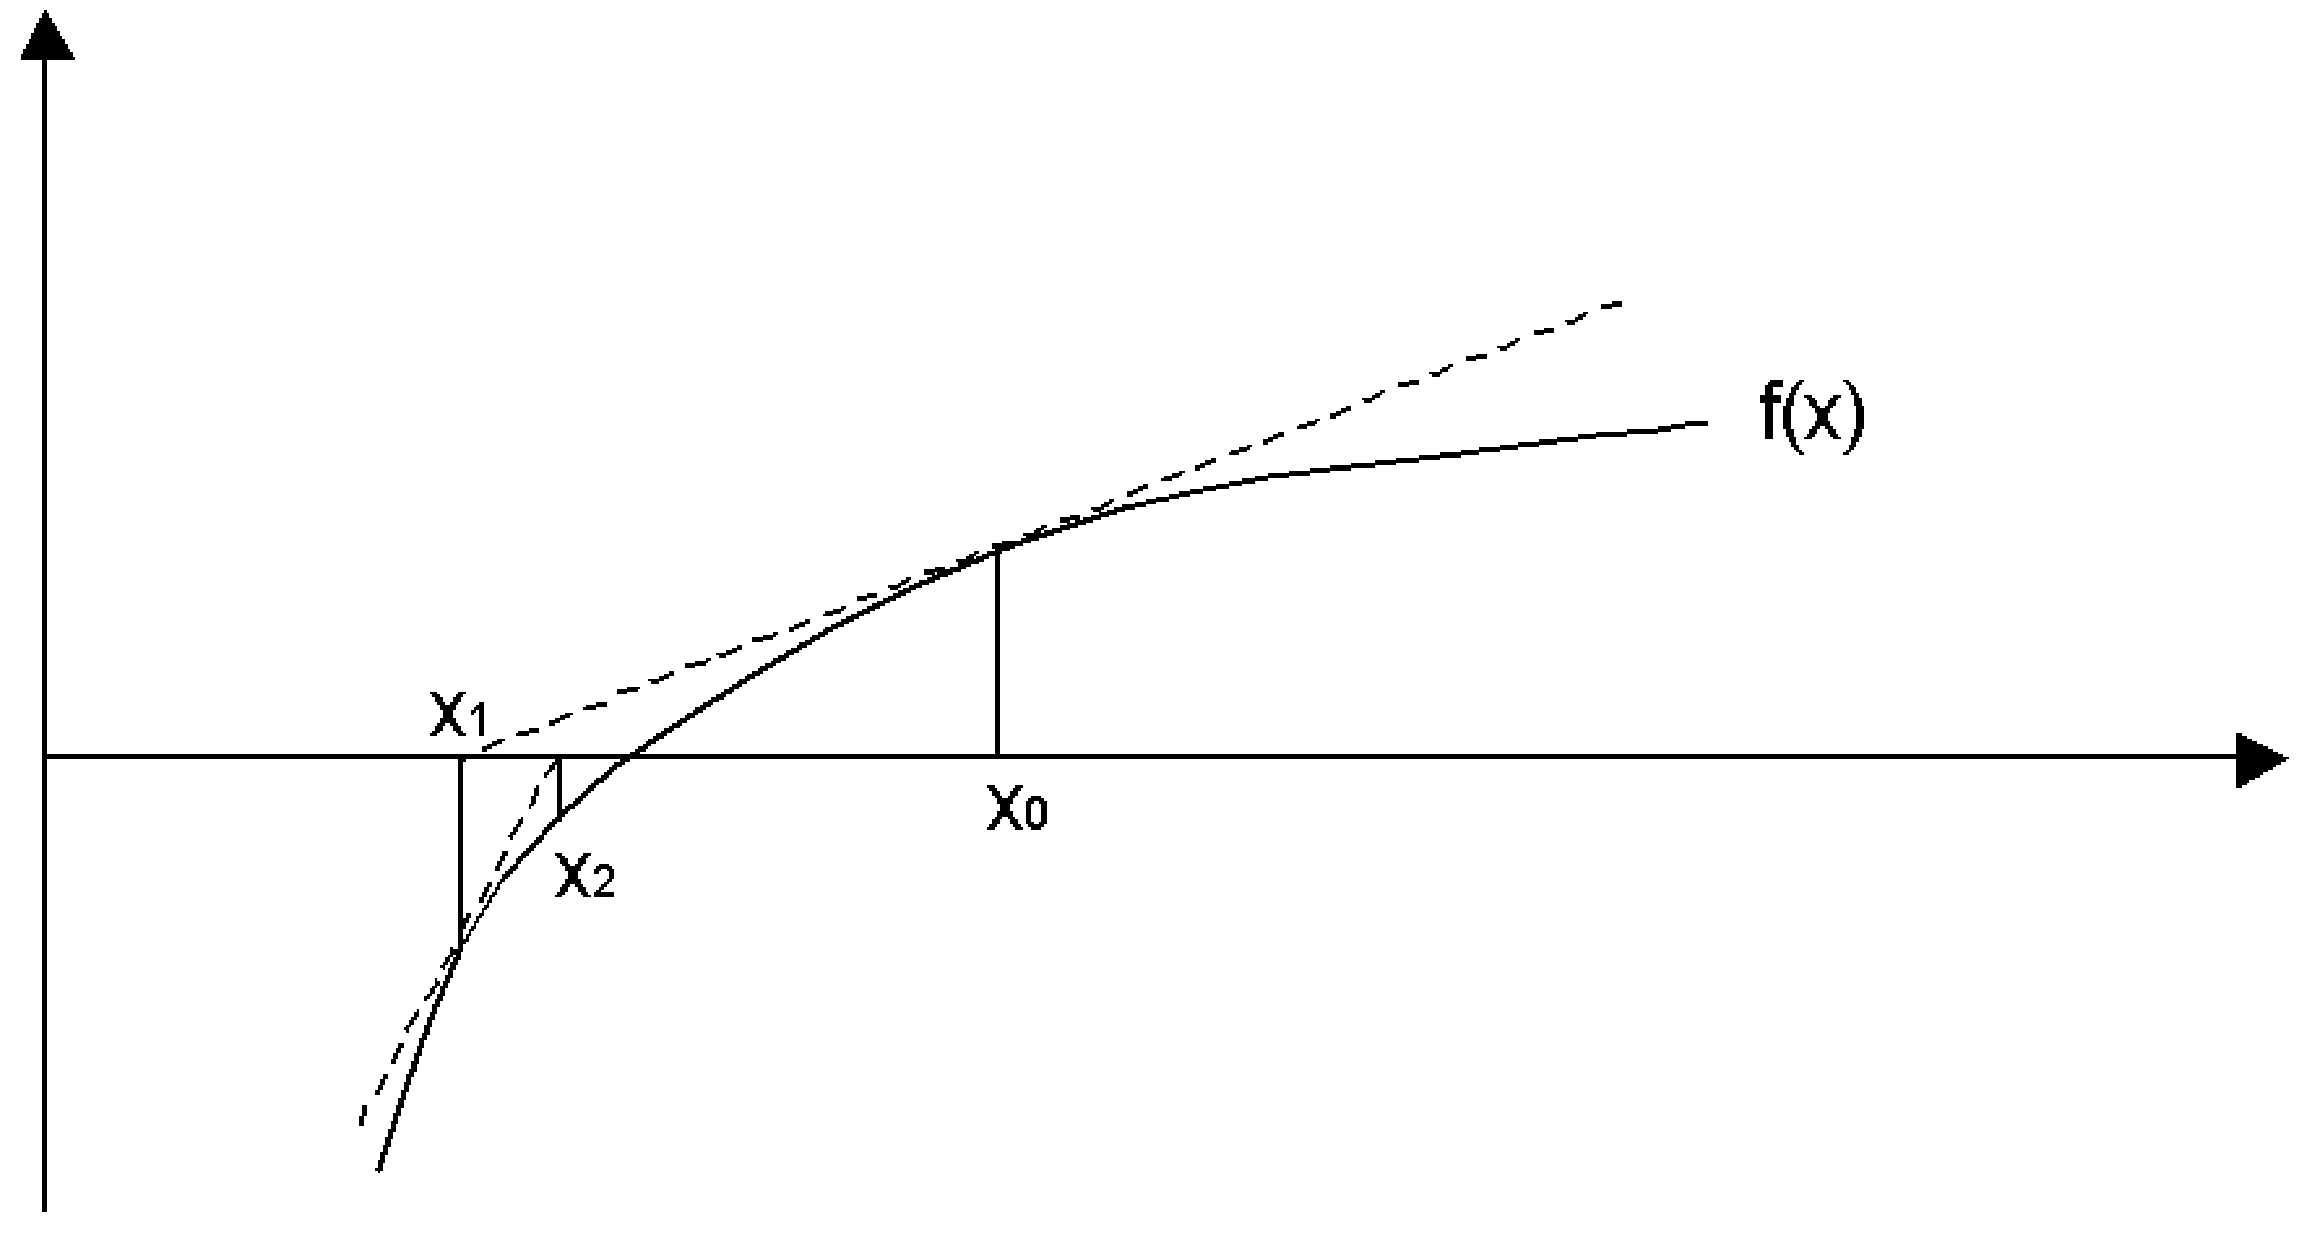
\includegraphics[width=12cm]{Figures/NewtonGraph}
\caption{Geometrical representation of Newton's zero finding
algorithm}\label{fig:newtonZero}
\end{figure}
\begin{equation}
  y=\left(x-x_n\right)\cdot f^{\prime}\left(x_n\right)+f\left(x_n\right)
\end{equation}
One can then see that $x_{n+1}$ is the point where the tangent to
the curve at the point $x_n$ crosses the $x$-axis. The algorithm
can be started at any point where the function's derivative is
non- zero.

The technique used in Newton's algorithm is a general technique
often used in approximations. The function is replaced by a linear
approximation\footnote{Mathematically, this corresponds to
estimate the function using the first two terms of its Taylor
series.}, that is a straight line going through the point defined
by the preceding value and its function's value. The slope of the
straight line is given by the first derivative of the function.
The procedure is repeated until the variation between the new
value and the preceding one is sufficiently small. We shall see
other examples of this technique in the remainder of this book
(\cf sections \ref{sec:lsfnonlin}, \ref{sec:mlfhist} and
\ref{sec:optimum}).

From equation \ref{eq:newtonZero}, one can see that the series may
not converge if $f^{\prime}\left(x\right)$ becomes zero. If the
derivative of the function is zero in the vicinity of the zero,
the bisection algorithm gives better results. Otherwise Newton's
algorithm is highly efficient. It usually requires 5-10 times less
iteration than the bisection algorithm. This largely compensates
for the additional time spent in computing the derivative.

The class implementing Newton's algorithm belongs to a subclass of
the functional iterator described in section \ref{sec:iterrel}. An
additional instance variable is needed to store the function's
derivative.

\subsection{Newton's method --- Smalltalk implementation}
\label{sec:snewton} Listing \ref{ls:newtonZero} shows the complete
implementation in Smalltalk. The class {\tt DhbNewtonZeroFinder}
is a subclass of the class {\tt DhbFunctionalIterator} described
in section \ref{sec:siterrel}. For example the following code
finds the solution of equation \ref{eq:centile90}.
\begin{codeExample}
\begin{verbatim}

| zeroFinder result |
zeroFinder:= DhbNewtonZeroFinder
            function: [ :x | x errorFunction - 0.9]
            derivative: [ :x | DhbErfApproximation new normal: x].
zeroFinder initialValue: 1.
result := zeroFinder evaluate.
zeroFinder hasConverged
\end{verbatim}
    {\tt ifFalse:[ {\sl <special case processing>}].}
\end{codeExample}
The second line creates the object responsible to find the zero
supplying the function and the derivative\footnote{As we have seen
in section \ref{sec:errorFunction}, the normal distribution is the
derivative of the error function.}. The third line defines the
starting value. The fourth line performs the algorithm and stores
the result if the algorithm has converged. The last two lines
check for convergence and take corrective action if the algorithm
did not converge.

The method {\tt computeInitialValues} is somewhat complex. First,
it checks whether the user supplied an initial value. If not, it
is assigned to 0. Then the method checks whether the user supplied
a derivative. If not a default derivative function is supplied as
a block closure by the method {\tt defaultDerivativeBlock}. The
supplied block closure implements the formula of equation
\ref{eq:derivative} (on page \pageref{eq:derivative}). If a
derivative is supplied, it is compared to the result of the
derivative supplied by default. This may save a lot of trouble if
the user made an error in coding the derivative. Not supplying a
derivative has some negative effect on the speed and limits the
precision of the final result. The method {\tt
initializeIterations} also checks whether the derivative is nearly
zero for the initial value. If that is the case, the initial value
is changed with a random walk algorithm. If no value can be found
such that the derivative is non-zero an error is generated.

If the function is changed, the supplied derivative must be
suppressed. Thus, the method {\tt setFunction:} must also force a
redefinition of the derivative. A method allows defining the
initial value. A creation method defining the function and
derivative is also supplied for convenience.

Like for the bisection, the algorithm itself is coded within the
method {\tt evaluateIteration}. Other methods needed by the
algorithm have been already implemented in the superclasses.
\begin{listing} Smalltalk implementation of Newton's zero-finding method \label{ls:newtonZero}
$$\halign{ #\hfil&\quad#\hfil\cr {\sl Class}& {\Large\bf DhbNewtonZeroFinder}\cr
{\sl Subclass of }&{\tt DhbFunctionalIterator}\cr\noalign{\vskip 1ex}

{\sl Instance variable names:}&\parbox[t]{4 in}{\tt  derivativeBlock }\cr\noalign{\vskip 1ex}}$$


Class methods
{\parskip 1ex\par\noindent}
{\bf function:} {\tt aBlock1} {\bf derivative:} {\tt aBlock2}
\begin{verbatim}
    ^(self new) setFunction: aBlock1; setDerivative: aBlock2; 
                                                              yourself

\end{verbatim}



Instance methods
{\parskip 1ex\par\noindent}
{\bf computeInitialValues}
\begin{verbatim}
    | n |
    result isNil
        ifTrue: [ result := 0].
    derivativeBlock isNil
        ifTrue: [ derivativeBlock := self defaultDerivativeBlock].
    n := 0.
    [ (derivativeBlock value: result) equalsTo: 0]
        whileTrue: [ n := n + 1.
                     n > maximumIterations
                        ifTrue: [ self error: 'Function''s derivative 
                                        seems to be zero everywhere'].
                     result := Number random + result].

\end{verbatim}
{\bf defaultDerivativeBlock}
\begin{verbatim}
    ^[ :x | 5000 * ( ( functionBlock value: (x + 0.0001)) - ( 
                                  functionBlock value: (x - 0.0001)))]

\end{verbatim}
{\bf evaluateIteration}
\begin{verbatim}
    | delta |
    delta := ( functionBlock value: result) / ( derivativeBlock 
                                                       value: result).
    result := result - delta.
    ^self relativePrecision: delta abs

\end{verbatim}
{\bf initialValue:} {\tt aNumber}
\begin{verbatim}
    result := aNumber.

\end{verbatim}
{\bf setDerivative:} {\tt aBlock}
\begin{verbatim}
    | x |
    ( aBlock respondsTo: #value:)
        ifFalse:[ self error: 'Derivative block must implement the 
                                                      method value:'].
    x := result ifNil: [ Number random] ifNot: [ :base | base + 
                                                       Number random].
    ( ( aBlock value: x) relativelyEqualsTo: (self 
                        defaultDerivativeBlock value: x) upTo: 0.0001)
        ifFalse:[ self error: 'Supplied derivative is not correct'].
    derivativeBlock := aBlock.

\end{verbatim}
{\bf setFunction:} {\tt aBlock}
\begin{verbatim}
    super setFunction: aBlock.
    derivativeBlock := nil.

\end{verbatim}


\end{listing}




\section{Example of zero-finding --- Roots of polynomials}
\label{sec:polroots} The zeroes of a polynomial function are
called the roots of the polynomial. A polynomial of degree $n$ has
at most $n$ real roots. Some\footnote{If the degree of the
polynomial is odd, there is always at least one non-complex root.
Polynomials of even degree may have only complex roots and no real
roots.} of them maybe complex, but are not covered in this book.

If $x_0$ is a root of the polynomial $P\left(x\right)$, then
$P\left(x\right)$ can be exactly divided by the polynomial
$x-x_0$. In other words there exists a polynomial
$P_1\left(x\right)$ such that:
\begin{equation}
\label{eq:rootdivide}
  P\left(x\right) = \left(x-x_0\right)\cdot P_1\left(x\right)
\end{equation}
Equation \ref{eq:rootdivide} also shows that all roots of
$P_1\left(x\right)$ are also roots of $P\left(x\right)$. Thus, one
can carry the search of the roots using recurrence. In practice a
loop is more efficient\footnote{The overhead comes from allocating
the structures needed by the method in each call.}. The process is
repeated at most $n$ times and will be interrupted if a zero
finding step does not converge.

One could use the division algorithm of section \ref{sec:polymath}
to find $P_1\left(x\right)$. In this case, however, the inner loop
of the division algorithm --- that is, the loop over the
coefficients of the dividing polynomial --- is not needed since
the dividing polynomial has only two terms. In fact, one does not
need to express $x-x_0$ at all as a polynomial. To carry the
division one uses a specialized algorithm taking the root as the
only argument. This specialized division algorithm is called {\sl
deflation} \cite{Press}.

Polynomials are very smooth so Newton's algorithm is quite
efficient for finding the first root. To ensure the best accuracy
for the deflation it is recommended to find the root of smallest
absolute value first. This works without additional effort since
our implementation of Newton's algorithm uses 0 at the starting
point by default. At each step the convergence of the zero-finder
is checked. If a root could not be found the process must be
stopped. Otherwise, the root finding loop is terminated when the
degree of the deflated polynomial becomes zero.

\subsection{Roots of polynomials --- Smalltalk implementation}
Roots of a polynomial can be obtained as an {\tt
OrderedCollection}. For example, the following code sample
retrieves the roots of the polynomial $x^3-2x^2-13x-10$:
\begin{codeExample}
\begin{verbatim}

\end{verbatim}
{\tt (DhbPolynomial coefficients: \#(-10 -13 -2 1)) roots}
\end{codeExample}
The methods needed to get the roots are shown in Listing
\ref{ls:polroots}.

The deflation algorithm is implemented in the method {\tt
deflateAt:} using the iterator method {\tt collect:} (\cf section
\ref{sec:collect}). An instance variable is keeping track of the
remainder of the division within the block closure used by the
method {\tt collect:}.

The roots are kept in an {\tt OrderedCollection} object
constructed in the method {\tt roots:}. The size of the {\tt
OrderedCollection} is initialize to the maximum expected number of
real roots. Since some of the roots may be complex, we are storing
the roots in an {\tt OrderedCollection}, instead of an {\tt
Array}, so that the number of found real roots can easily be
obtained. This method takes as argument the desired precision used
in the zero finding algorithm. A method root uses the default
numerical machine precision as discussed in section
\ref{sec:findprecision}.

\begin{listing} Smalltalk implementation of finding the roots of a polynomial \label{ls:polroots}
$$\halign{ #\hfil&\quad#\hfil\cr {\sl Class}& {\Large\bf DhbPolynomial}\cr
{\sl Subclass of }&{\tt Object}\cr\noalign{\vskip 1ex}

{\sl Instance variable names:}&\parbox[t]{4 in}{\tt  coefficients }\cr\noalign{\vskip 1ex}}$$


Instance methods
{\parskip 1ex\par\noindent}
{\bf deflatedAt:} {\tt aNumber}
\begin{verbatim}
    | remainder next newCoefficients|
    remainder := 0.
    newCoefficients := coefficients collect:
                        [ :each |
                          next := remainder. 
                          remainder := remainder * aNumber + each.
                          next].
    ^self class new: ( newCoefficients copyFrom: 2 to: 
                                         newCoefficients size) reverse

\end{verbatim}
{\bf roots}
\begin{verbatim}
    ^self roots: DhbFloatingPointMachine new 
                                             defaultNumericalPrecision

\end{verbatim}
{\bf roots:} {\tt aNumber}
\begin{verbatim}
    | pol roots x rootFinder |
    rootFinder := DhbNewtonZeroFinder new.
    rootFinder desiredPrecision: aNumber.
    pol := self class new: ( coefficients reverse collect: [ :each | 
                                                       each asFloat]).
    roots := OrderedCollection new: self degree.
    [ rootFinder setFunction: pol; setDerivative: pol derivative.
      x := rootFinder evaluate.
      rootFinder hasConverged
        ] whileTrue: [ roots add: x. 
                       pol := pol deflatedAt: x. 
                       pol degree > 0
                         ifFalse: [ ^roots].
                     ].
    ^roots

\end{verbatim}


\end{listing}

\section{Which method to choose}
There are other zero-finding techniques: {\it regula falsi}, Brent
\cite{Press}. For each of these methods, however, a specialist of
numerical methods can design a function causing that particular
method to fail.

In practice the bisection algorithm is quite slow as can be seen
from equation \ref{eq:bissectime}. Newton's algorithm is faster
for most functions you will encounter. For example, it takes 5
iterations to find the zero of the logarithm function with
Newton's algorithm to a precision of $3\cdot 10^{-9}$ whereas the
bisection algorithm requires 29 to reach a similar precision. On
the other hand bisection is rock solid and will always converge
over an interval where the function has no singularity. Thus, it
can be used as a recovery when Newton's algorithm fails.

My own experience is that Newton's algorithm is quite robust and
very fast. It should suffice in most cases. As we have seen
Newton's algorithm will fail if it encounters a value for which
the derivative of the function is very small. In this case, the
algorithm jumps far away from the solution. For these cases, the
chances are that the bisection algorithm will find the solution if
there is any. Thus, combining Newton's algorithm with bisection is
the best strategy if you need to design a foolproof algorithm.

Implementing an object combining both algorithms is left as an
exercise to the reader. Here is a quick outline of the strategy to
adopt. Newton's algorithm must be modified to keep track of values
for which the function takes negative values and positive values
--- that is the values $x_{\mathop{\rm pos}}$ and $x_{\mathop{\rm neg}}$
--- making sure that the value $\left| x_{\mathop{\rm pos}}-x_{\mathop{\rm neg}}\right|$
never increases. Then, at each step, one must check that the
computed change does not cause the solution to jump outside of the
interval defined by $x_{\mathop{\rm pos}}$ and $x_{\mathop{\rm
neg}}$. If that is the case, Newton's algorithm must be
interrupted for one step using the bisection algorithm.

\ifx\wholebook\relax\else\end{document}\fi
